\chapter{Arquitectura de \emph{Internet of Things}}

\section{Simulación de parámetros de red inalámbrica}
\begin{itemize}
	\item Instale el simulador de redes ns3
	\item en ns-3.26 /examples/stats puede encontrar un buen ejemplo de un proceso de simulación que incluye:
	\begin{itemize}
		\item una topología inalámbrica (wifi-example-sim.cc)
		\item La topología define dos nodos con una interfaz 802.11 cada uno. Ambos nodos se comunican por medio de un canal inalámbrico enviando paquetes pertenecientes a una aplicación (wifi-example-apps.cc/h)
		\item la simulación cambia varios argumentos desde la linea de comandos. El parámetro principal es la distancia entre ambos nodos.
		\item la simulación almacena los resultados de la simulación en una base de datos sqlite3.
		\item el script wifi-example-db.sh ejecuta varias veces la simulación alejando los nodos.
		\item después de la simulación se resume en el archivo wifi-default.data la pérdida de paquetes
		\item se dibuja el gráfico con la herramienta gnuplot.
	\end{itemize}
\begin{figure}
	\centering
	\includegraphics[width=0.7\linewidth]{figures/wifi-default.eps}
	\caption{Distancia entre nodos en metros vs porcentaje de paquetes perdidos}
	\label{fig:wifi}
\end{figure}
	\item Ejecute el ejemplo, debería obtener la figura ~\ref{fig:wifi}.
	\item Cambie el script e incremente las distancias a simular 25 50 75 100 125 145 147
	150 152 155 157 160 162 165 167 170 172 175 177 180 185 190 195 200 210 220 230 240 250
	300 350 400 450 500 600 750 1000
	\item reduzca el número de simulaciones por cada distancia de 5 a 1
	\item ajuste el eje x para mostrar las nuevas simulaciones en el script gnuplot.
	\item 
\end{itemize}

A continuación vamos a cambiar la simulación propiamente dicha. Para el siguiente código:
\begin{verbatim}
1  NodeContainer nodes;
2  nodes.Create (2);

3  NS_LOG_INFO ("Installing WiFi and Internet stack.");
4  WifiHelper wifi = WifiHelper::Default ();

5  NqosWifiMacHelper wifiMac = NqosWifiMacHelper::Default ();
6  wifiMac.SetType ("ns3::AdhocWifiMac");
7  YansWifiPhyHelper wifiPhy = YansWifiPhyHelper::Default ();
8  YansWifiChannelHelper wifiChannel = YansWifiChannelHelper::Default ();
9   wifiPhy.SetChannel (wifiChannel.Create ());
10  NetDeviceContainer nodeDevices = wifi.Install (wifiPhy, wifiMac, nodes);
\end{verbatim}

\begin{itemize}
	\item ¿Qué objeto representa la antena?¿Qué propiedades se deberían cambiar para incrementar el rango de comunicaciones?
	\item Cambie los parámetros de la antena necesarios para tener una comunicación satisfactoria a 400 metros. Muestre el gráfico con la nueva simulación.
\end{itemize}

Como podemos observar el cambio entre 0\% paquetes perdidos y 100\% es bastante brusco. Existen implementados diferentes modelos de propagación. Vamos 
a cambiar el modelo de propagación (linea 8). Para ello:
\begin{itemize}
	\item Elimine la modificación realizada anteriormente para tener los parámetros por defecto de la antena (con rango de comunicación 100 metros)
	\item Incremente el número de simulaciones en la distancia clave donde el número de paquetes empieza a perderse. Por ejemplo de 10 metros en 10 metros entre 90 y 180 metros.
	\item Pruebe otro modelo de propagación (compruebe el método AddPropagationLoss de la clase YansWifiChannelHelper) y muestre un gráfico comparando el resultado de YansWifiChannel con el modelo de propagación por defecto y el modelo de propagación escogido por usted.  
\end{itemize}

\section{Diseño de arquitectura de aplicaciones}
Para las siguientes aplicaciones, esboce la arquitectura del sistema, proponga un nodo/Tecnología de conectividad/pasarela. Analice el coste de la solución propuesta en cuanto al hardware.
\begin{itemize}
\item Localización de ganado bobino en áreas rurales con el objeto de análisis de patrones de comportamiento (localización). El punto de control se encuentra en la propia granja.
\item Monitorización de flujos de agua subterráneas (tuberías) en ciudades para evitar pérdidas. El punto de control se encuentra en el ayuntamiento.
\item Monitorización de plazas de parking libres en un gran supermercado. El punto de control se encuentra en el supermercado. Los usuarios acceden a dicha información mediante una app.
\item Monitorización de cuencas fluviales de ríos El ministerio de agricultura recolecta toda la información.
\item Gestión inteligente de tráfico (control de semáforos, sensores de tráfico, señalización inteligente, etc.) El ayuntamiento analiza la información, la interacción entre semáforos, tráfico y señalización inteligente es entre el vehículo y la infraestructura.
\end{itemize}

\section{Configuración de la Pasarela/s}
\begin{itemize}
\item Como forma de tolerancia a fallos, usted decide poner tres pasarelas entre su red IoT e Internet.
  \begin{itemize}
  \item ¿Cómo evito que me lleguen los mensajes por triplicado?
  \item ¿Necesito enviar tres mensajes distintos desde un sensor?
  \item ¿Cómo compruebo que todos los nodos están vivos? ¿Es escalable esta solución?
  \item Una pasarela con una limitación de un 1\% \emph{duty cycle} y que sólo envía ACKs de 10 ms, ¿cuantos ACK puede mandar en un día?, ¿cómo limita este número al número de dispositivos que puede atender una única pasarela? ¿Cuantos dispositivos puede atender la pasarela si cada dispositivo envía 10 mensajes a la hora?
  \end{itemize}
\end{itemize}

\section{MQTT}
\begin{itemize}
	\item Atendiendo a la dirección de red del broker MQTT, envíe un mensaje a Argentina/SanLuis/USL/master con su nombre completo.
	\item 5 clientes denominados A,B,C,D y E se han subscrito a los eventos MQTT en los siguientes canales:
	\begin{itemize}
		\item Cliente A: Argentina/
		\item Cliente B: Argentina/SanLuis
		\item Cliente C: Argentina/SanLuis/calleluis
		\item Cliente D: Argentina/sanLuis/calleluis
		\item Cliente E: Argentina/SanLuis/calleluis/4
	\end{itemize} 
	\item para los subscriptores anteriores, publique un mensaje con contenido "on" en los siguientes canales e indique qué clientes lo reciben:
	\begin{itemize}
		\item /Argentina
		\item Argentina/\#
		\item Argentina/?/calleluis
		\item Argentina/?
		\item Argentina/SanLuis/?
		\item Argentina
		\item ?/\#
		\item \#/?
		\item \#
		\item ?
	\end{itemize}
\end{itemize}

\section{Gestión de topologías Ad-Hoc}
Las redes de sensores inalámbricas son unas redes formadas por nodos de bajo coste dotados con una tecnología inalámbrica (por ejemplo 802.15.4e). Una de las configuraciones mas habituales de ese tipo de redes es la comunicación multisalto. Esta configuración es usada para extender el alcance de comunicación de cada uno de los nodos gracias a que cada uno de los nodos enruta la información del resto hacia la pasarela. La pasarela envía toda la información a través de un interfaz mas apropiado (por ejemplo, un modem LTE). El problema es que un nodo sólo puede enrutar tráfico estando en estado DESPIERTO ya que en estado DORMIDO no recibe ningún tipo de mensaje. De forma adicional, un nodo constantemente DESPIERTO consume mucha batería por lo que hay que mantener el mínimo número de nodos despiertos imprescindible para que la información pueda llegar a la pasarela. Se le pide que diseñe un algoritmo a ejecutar en cada uno de los nodos de la red, de forma que:
\begin{itemize}
\item Al final de la ejecución del algoritmo, un nodo decida si está DESPIERTO o DORMIDO.
\item Un nodo DORMIDO se despierta regularmente y envía la lectura de su sensor (por ejemplo, temperatura) a un nodo qué, para que reciba su mensaje, tiene que estar  DESPIERTO.
\item Un nodo DESPIERTO tiene a todos sus vecinos dormidos excepto a uno que se encuentra mas cerca de la pasarela y le servirá para enviar la información a la pasarela.  Un vecino de un nodo es un nodo con el cual tiene enlace directo. 
\end{itemize}
En la figura~\ref{fig:adhoc} vemos una red de sensores inalámbrica donde cada nodo viene representado por un círculo y cada enlace inalámbrico directo viene representado por una linea. Si cada uno de los nodos  ejecuta su algoritmo, los nodos tomarán una decisión de si se quedan despiertos o dormidos formando un camino hacia la pasarela. Por ejemplo, en la red de la figura una posible solución sería la que se representa en la figura de abajo con los nodos que han decidido quedarse despiertos en negro.
Como consejo para el desarrollo del algoritmo, comience con redes simples (dos o tres nodos) conectados a una pasarela y trate de dibujar a mano el intercambio de mensajes necesario para que esa red simple logre el objetivo planteado. Trate de extender ese primer algoritmo a redes mas complejas.
Debe entregar el pseudocodigo de la solución.

\begin{figure}
	\centering
	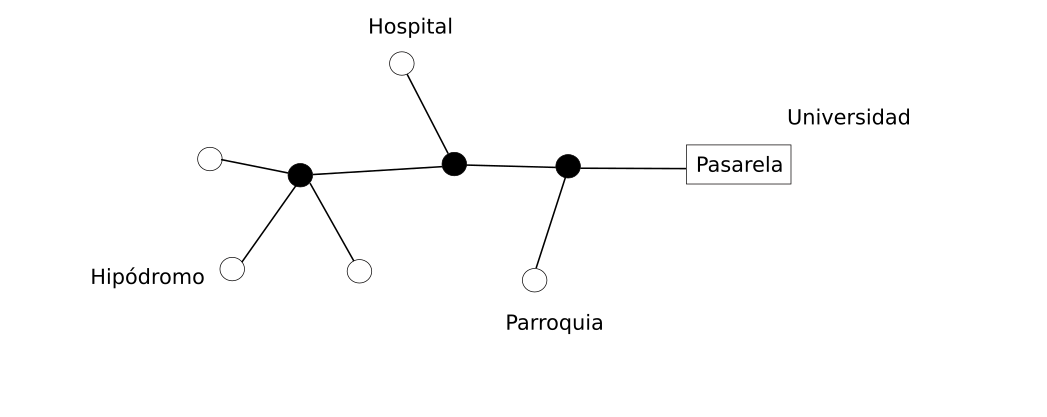
\includegraphics[width=0.7\linewidth]{figures/adhoc.png}
	\caption{Ejecución algoritmo, los nodos en negro deciden quedarse despiertos, los nodos en blanco, dormidos}
	\label{fig:adhoc}
\end{figure}



% Local Variables:
%   coding: utf-8
%   fill-column: 90
%   mode: flyspell
%   ispell-local-dictionary: "spanish"
%   mode: latex
%   TeX-master: "main"
% End:
